\documentclass{article}
\usepackage[utf8]{inputenc}
\usepackage[spanish]{babel}
\usepackage{graphicx}
\usepackage{hyperref}
\usepackage{geometry}
\usepackage{booktabs}
\usepackage{longtable}
\usepackage{array}
\usepackage{xcolor}
\usepackage{textcomp}
\geometry{margin=2.5cm}

\title{Proyecto InfoVis \textbf{Grupo 11}}
\author{Jos\'{e} Garc\'{i}a, Daniel Rojas, Sergio Hern\'{a}ndez y Edgardo Jara}
\date{Octubre 2026}

\begin{document}

\maketitle

% =========================================================
\section*{Portada}
% =========================================================

\begin{center}
  \Large\textbf{Grupo 11} \\[0.5em]
  \normalsize
  Jos\'{e} Garc\'{i}a \quad Daniel Rojas \quad Sergio Hern\'{a}ndez \quad Edgardo Jara \\[1em]
  \begin{tabular}{ll}
    \textbf{GitHub Pages:}  & \url{https://josegdotcom.github.io/Proyecto-infovis/} \\[0.3em]
    \textbf{Repositorio:}   & \url{https://github.com/josegdotcom/Proyecto-infovis} \\[0.3em]
    \textbf{Video:}         & {[SECCION PENDIENTE]} \\
  \end{tabular}
\end{center}

\newpage
\tableofcontents
\newpage

% =========================================================
\section{Contexto general}
% =========================================================

\subsection{Mensaje principal}

\textit{
Las inteligencias artificiales son percibidas como herramientas perfectas y universales, pero
esa percepci\'{o}n es errada.
Para demostrarlo, entrenamos dos redes neuronales ---una convolucional (CNN) y una de
propagaci\'{o}n densa (MLP)--- y las pusimos a prueba en dos tareas distintas: clasificar
dibujos de gatos y perros (datos de imagen) y reconocer actividades humanas a partir del
girosc\'{o}pio del tel\'{e}fono (datos tabulares).
La CNN destaca en im\'{a}genes; la MLP entrena m\'{a}s r\'{a}pido en ambas pruebas y
obtiene mejores resultados en actividades.
El objetivo es mostrar que cada modelo tiene sus fortalezas y limitaciones seg\'{u}n el
tipo de dato que procesa.
}

\subsection{Origen y procesamiento de los datos}

Los datos provienen de dos fuentes abiertas:
\textbf{Quick, Draw!} (Google) para los dibujos de gatos y perros, y
\textbf{Human Activity Recognition Using Smartphones} (UCI) para los registros de
acel\'{e}r\'{o}metro y girosc\'{o}pio.
Los dibujos se almacenaron en \texttt{gatos\_perros\_dataset.npz} y se procesaron mediante el
notebook \texttt{data/Prueba\_1.ipynb}; los datos de actividades en \texttt{har\_dataset.npz}
mediante \texttt{data/Prueba\_2.ipynb}.
Los resultados se exportaron a archivos CSV/NPZ en \texttt{data/resultados/} y luego a
\texttt{exploracion/datos.js} para ser consumidos por la visualizaci\'{o}n web.

% =========================================================
\section{V1 --- la idea completa}
% =========================================================

\subsection{Identificaci\'{o}n}

\begin{tabular}{ll}
  \textbf{Fecha:}  & 28 de septiembre de 2026 \\
  \textbf{Commit:} & \texttt{329aa99} --- Merge PR \#1 (feature-NewIdea) \\
\end{tabular}

\subsection{Evidencia}

\begin{center}
  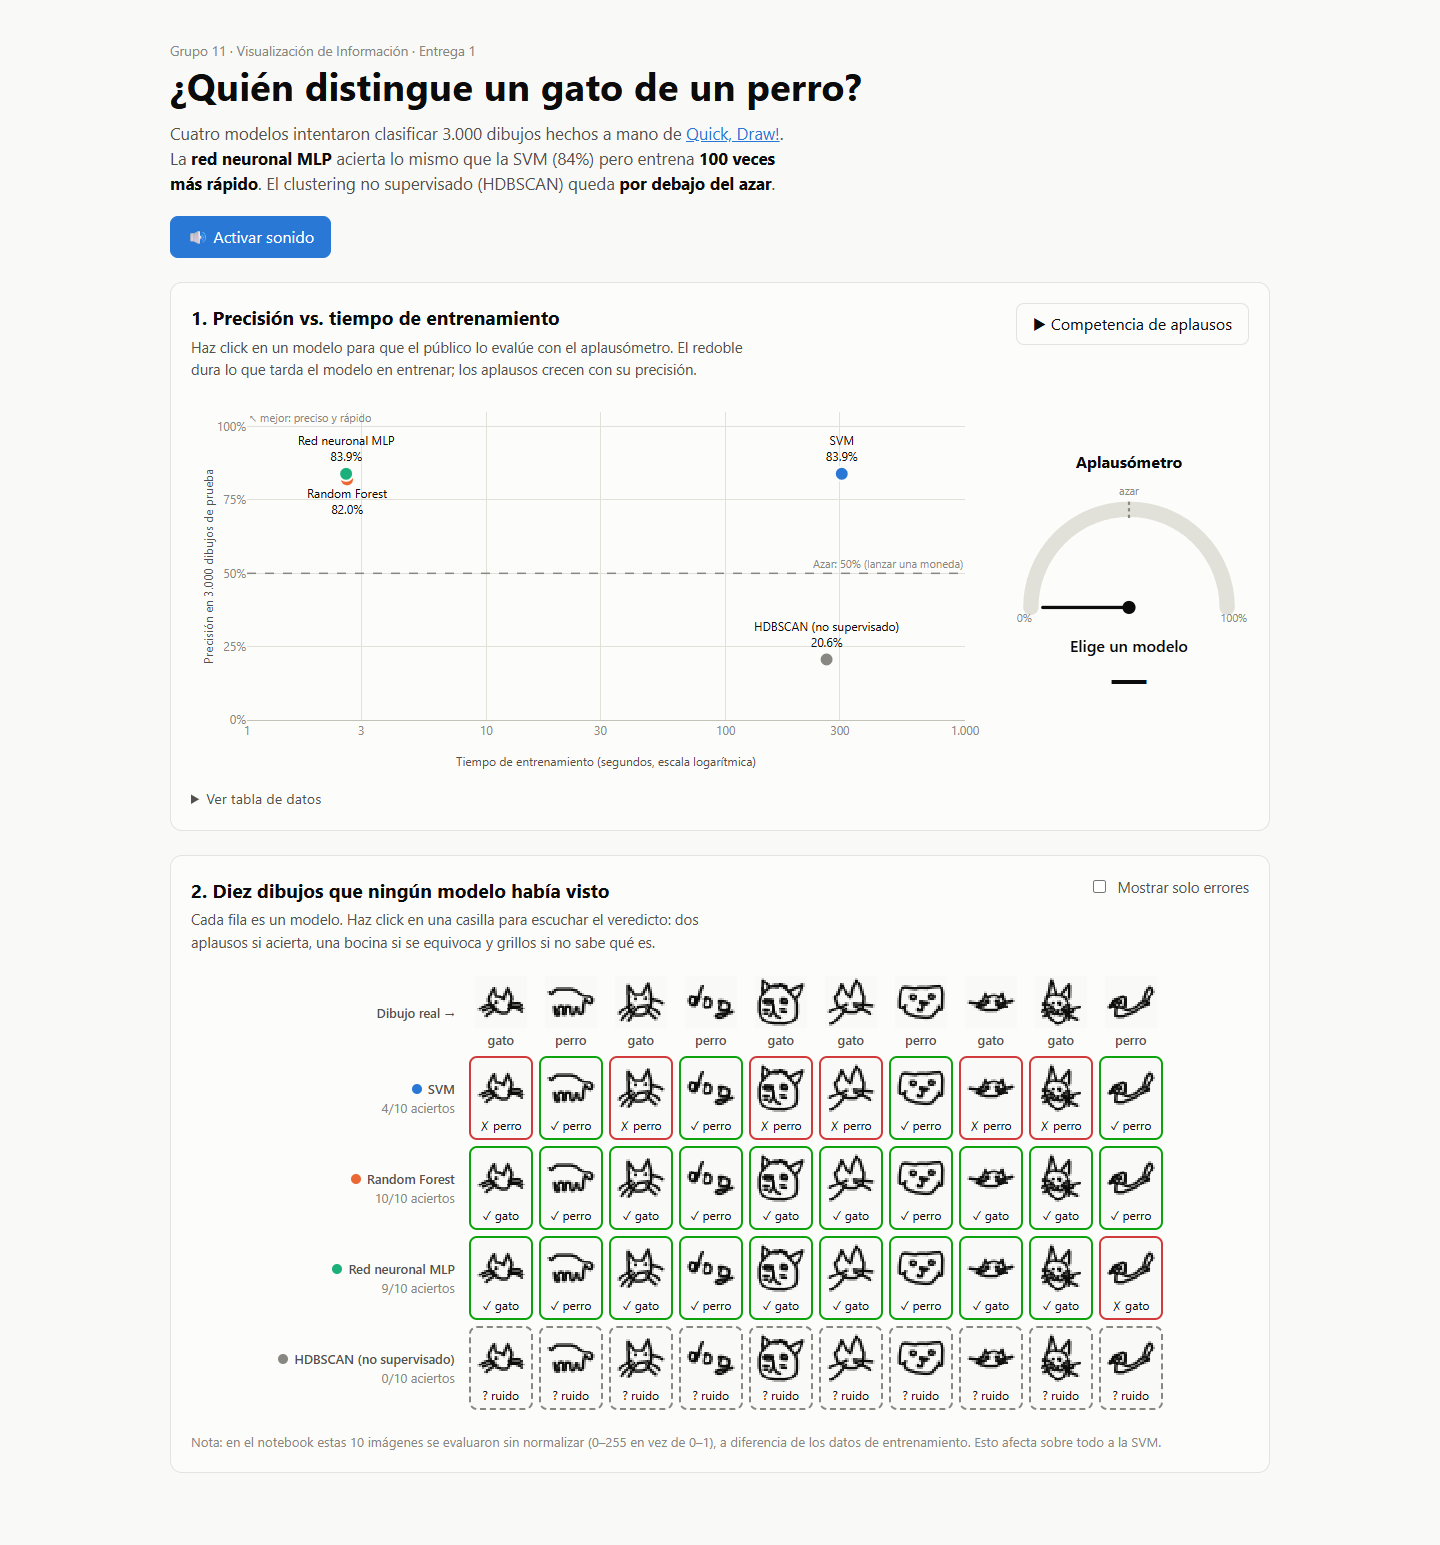
\includegraphics[width=0.8\linewidth]{evidencia2/V1/v1_pagina_completa.png}
\end{center}

\begin{center}
  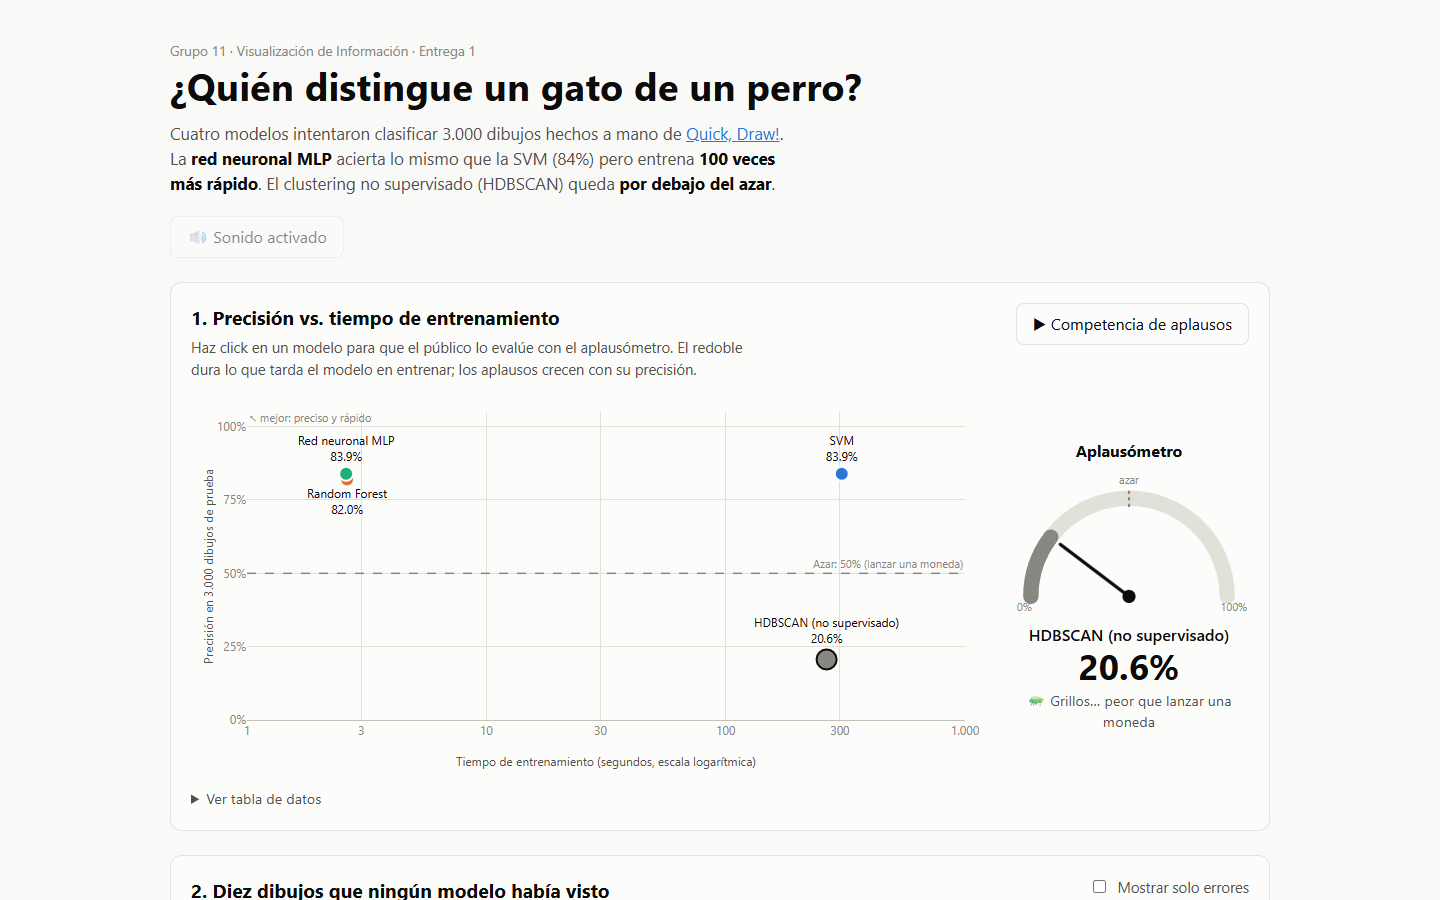
\includegraphics[width=\linewidth]{evidencia2/V1/v1_aplausometro.png}
\end{center}

\begin{center}
  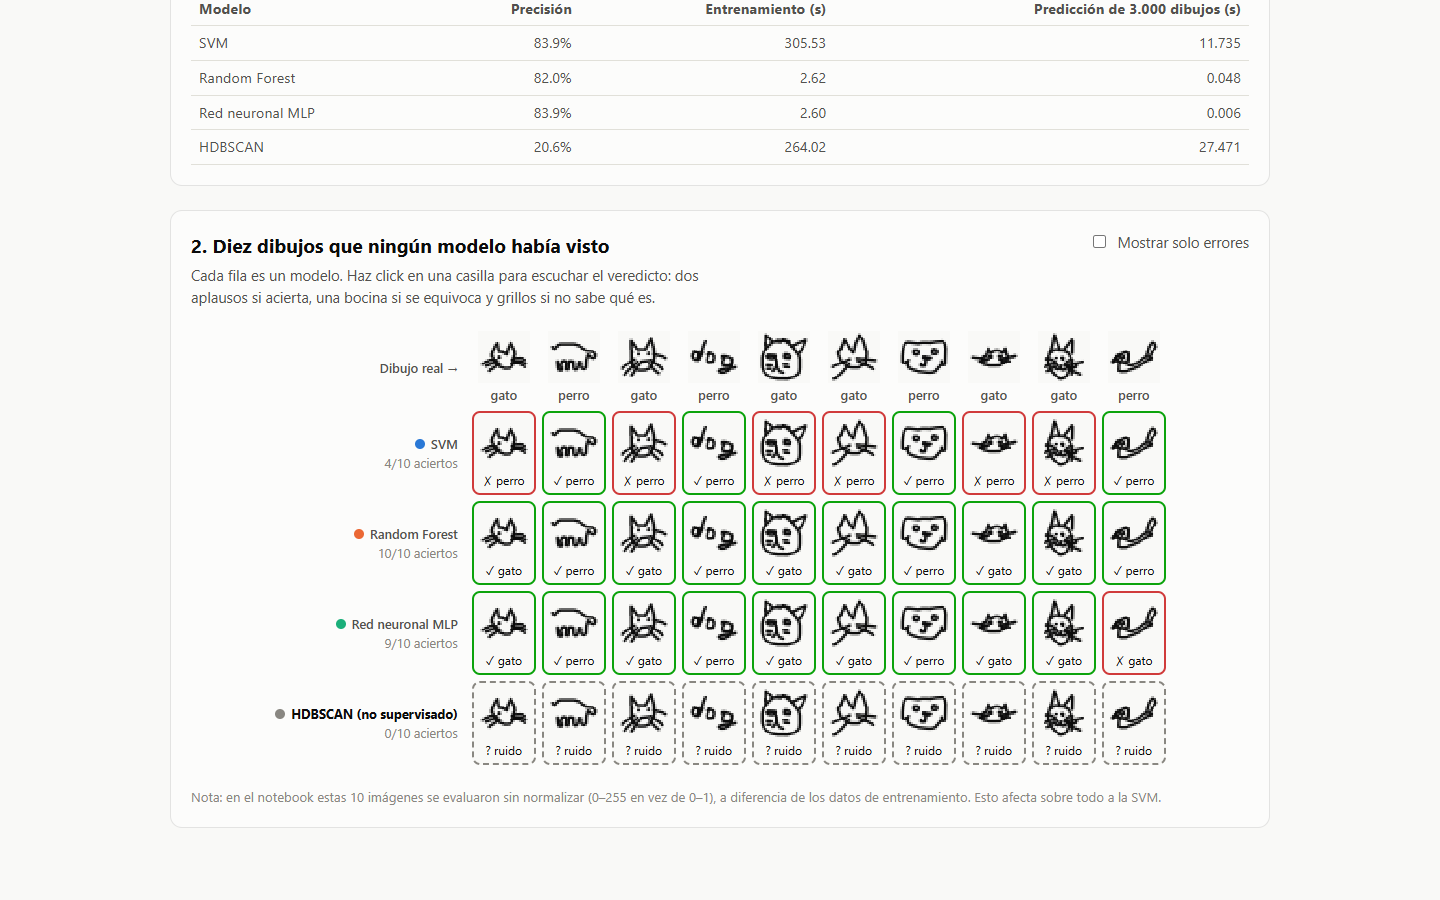
\includegraphics[width=\linewidth]{evidencia2/V1/v1_grilla.png}
\end{center}

\noindent\textbf{Video} (click en la imagen para reproducirlo):
\begin{center}
  \href{https://josegdotcom.github.io/Proyecto-infovis/evidencia2/V1/v1_video.mp4}{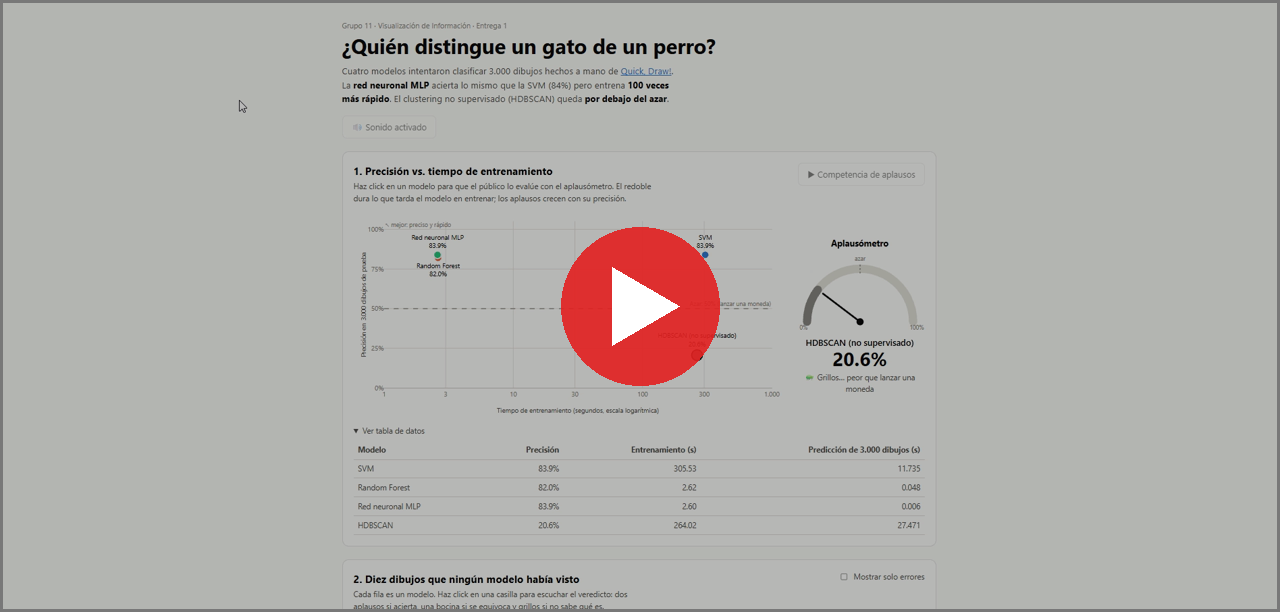
\includegraphics[width=0.85\linewidth]{evidencia2/V1/v1_video_miniatura.png}}\\[0.3em]
  \small\url{https://josegdotcom.github.io/Proyecto-infovis/evidencia2/V1/v1_video.mp4}
\end{center}

\subsection{Qu\'{e} cambi\'{o}}

Se descart\'{o} la idea original (basada en datos de mesas operativas electorales) y se adopt\'{o}
el concepto definitivo: comparar CNN y MLP en dos tipos de datos.
Se incorporaron ambos datasets, se construy\'{o} el gr\'{a}fico interactivo con un
``aplaus\'{o}metro'' y se agregaron los primeros sonidos (ca\'{i}da de fruta).
La p\'{a}gina principal (\texttt{index.html}) pas\'{o} de esqueleto vac\'{i}o a
visualizaci\'{o}n funcional.

\subsection{Por qu\'{e} cambi\'{o} (rationale)}

La idea original no ten\'{i}a un mensaje claro ni datos que permitieran una visualizaci\'{o}n
suficientemente rica.
El nuevo concepto permit\'{i}a incorporar dos dimensiones (aciertos y tiempo de entrenamiento)
m\'{a}s una distinci\'{o}n entre tipos de datos, abriendo espacio para sonificaci\'{o}n y
narrativa visual.
El cambio fue impulsado por la necesidad de comunicar un mensaje concreto y verificable.

\subsection{Qu\'{e} se descart\'{o}}

Se descart\'{o} el dataset de mesas operativas electorales y el concepto original basado en
\'{e}l. Tambi\'{e}n se elimin\'{o} el notebook \texttt{data/generador.ipynb} de la idea previa.

% =========================================================
\section{R1 --- revisi\'{o}n con el equipo docente}
% =========================================================

\begin{tabular}{ll}
  \textbf{Fecha:} & {[SECCION PENDIENTE]} \\
\end{tabular}

\medskip
\noindent\textbf{S\'{i}ntesis de lo discutido:}

{[SECCION PENDIENTE]}

\medskip
\noindent\textbf{Decisiones tomadas:}

{[SECCION PENDIENTE]}

% =========================================================
\section{V2 --- primera iteraci\'{o}n de dise\~{n}o}
% =========================================================

\subsection{Identificaci\'{o}n}

\begin{tabular}{ll}
  \textbf{Fecha:}  & 7 de octubre de 2026 \\
  \textbf{Commit:} & \texttt{b878af6} --- Merge PR \#2 (feature-variacion\_datos\_train) \\
\end{tabular}

\subsection{Evidencia}

\begin{center}
  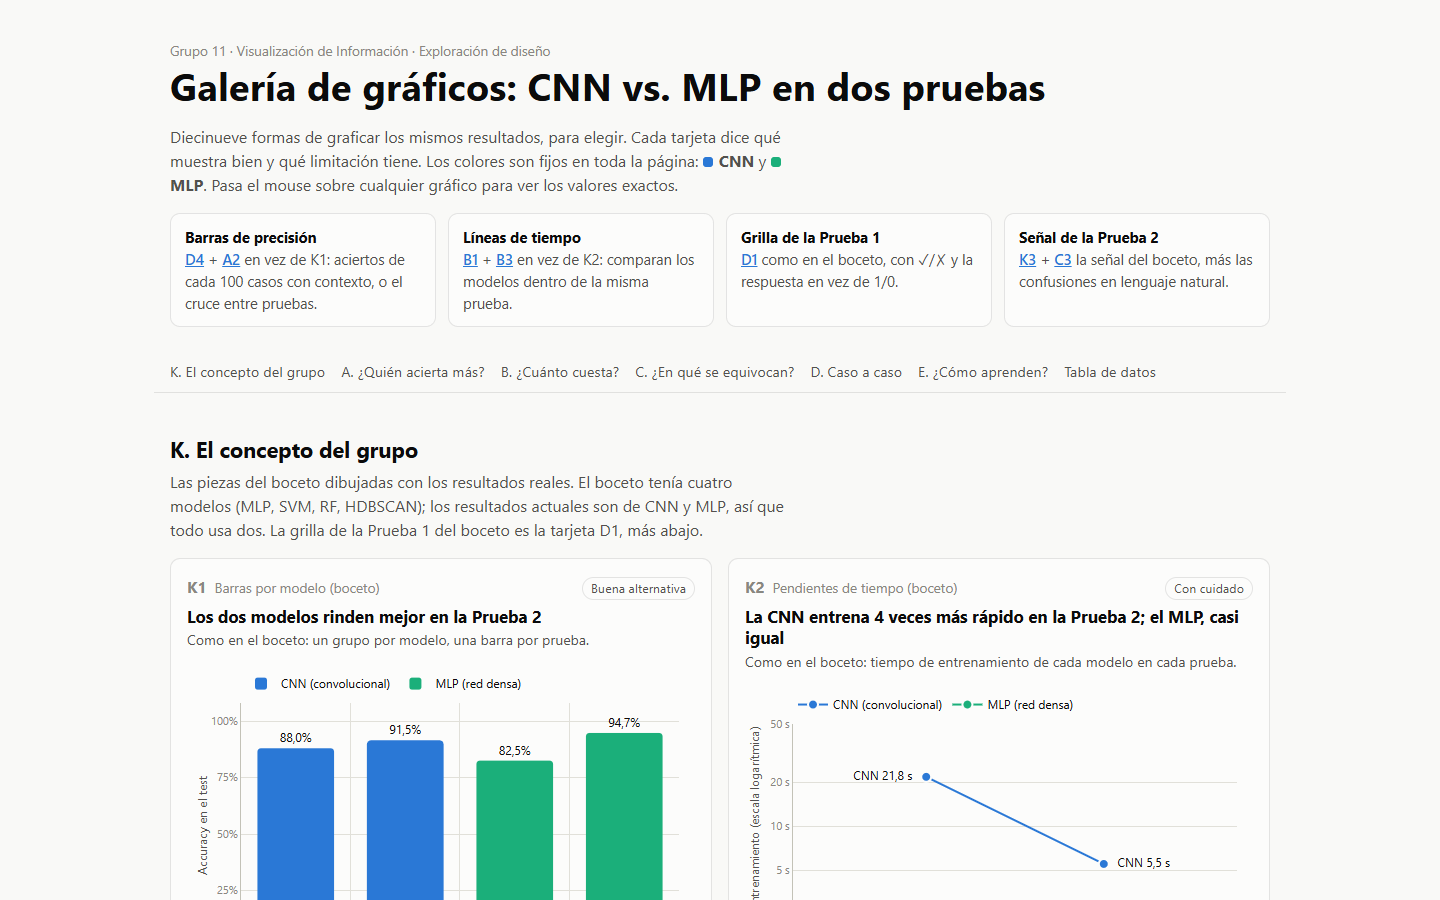
\includegraphics[width=\linewidth]{evidencia2/V2/v2_galeria_inicio.png}
\end{center}

\begin{center}
  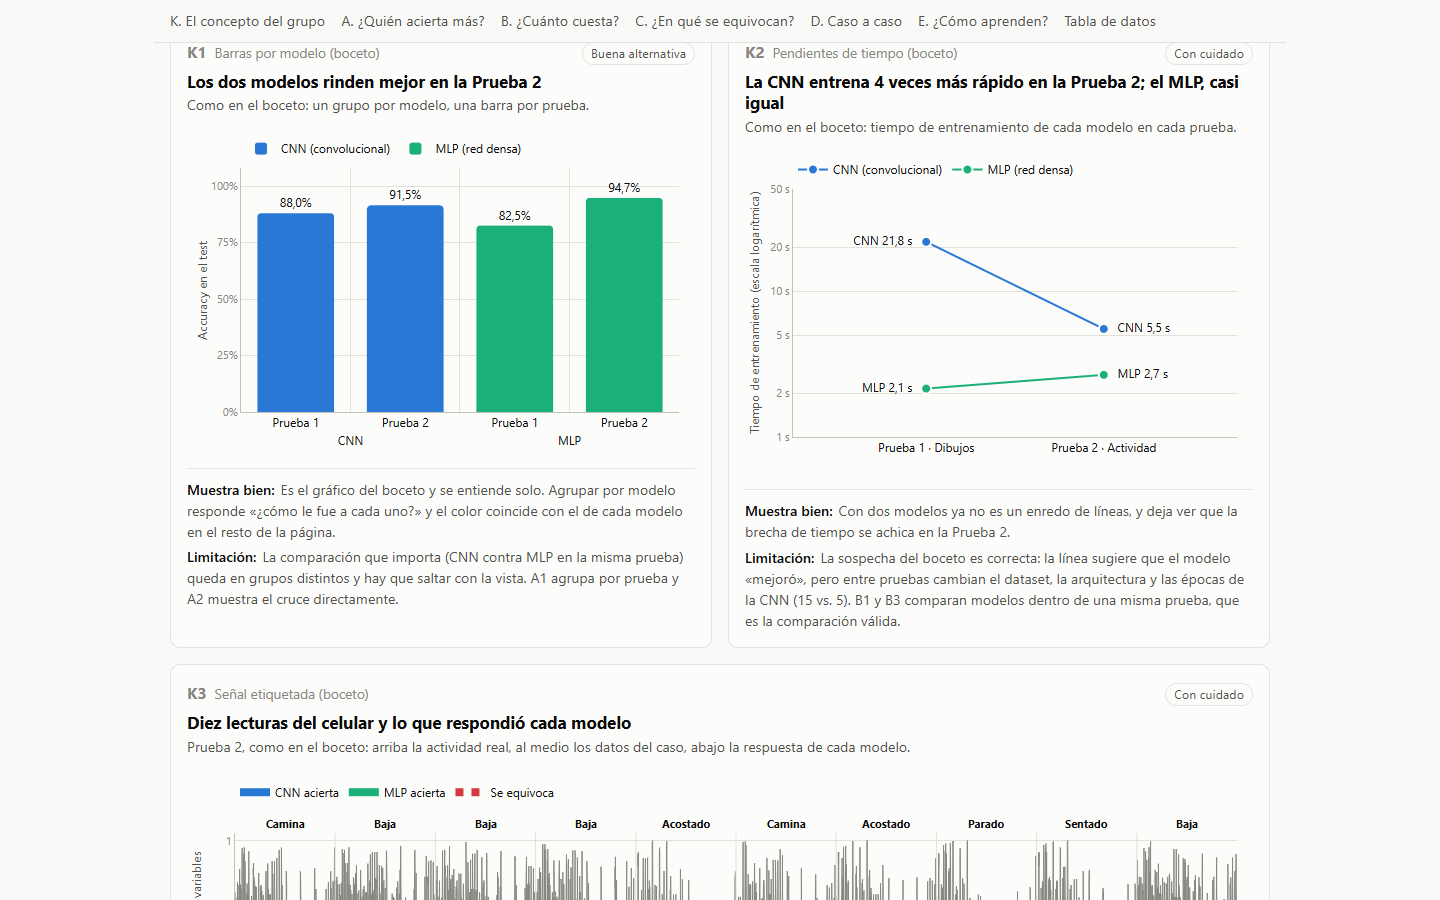
\includegraphics[width=\linewidth]{evidencia2/V2/v2_seccion_k.png}
\end{center}

\begin{center}
  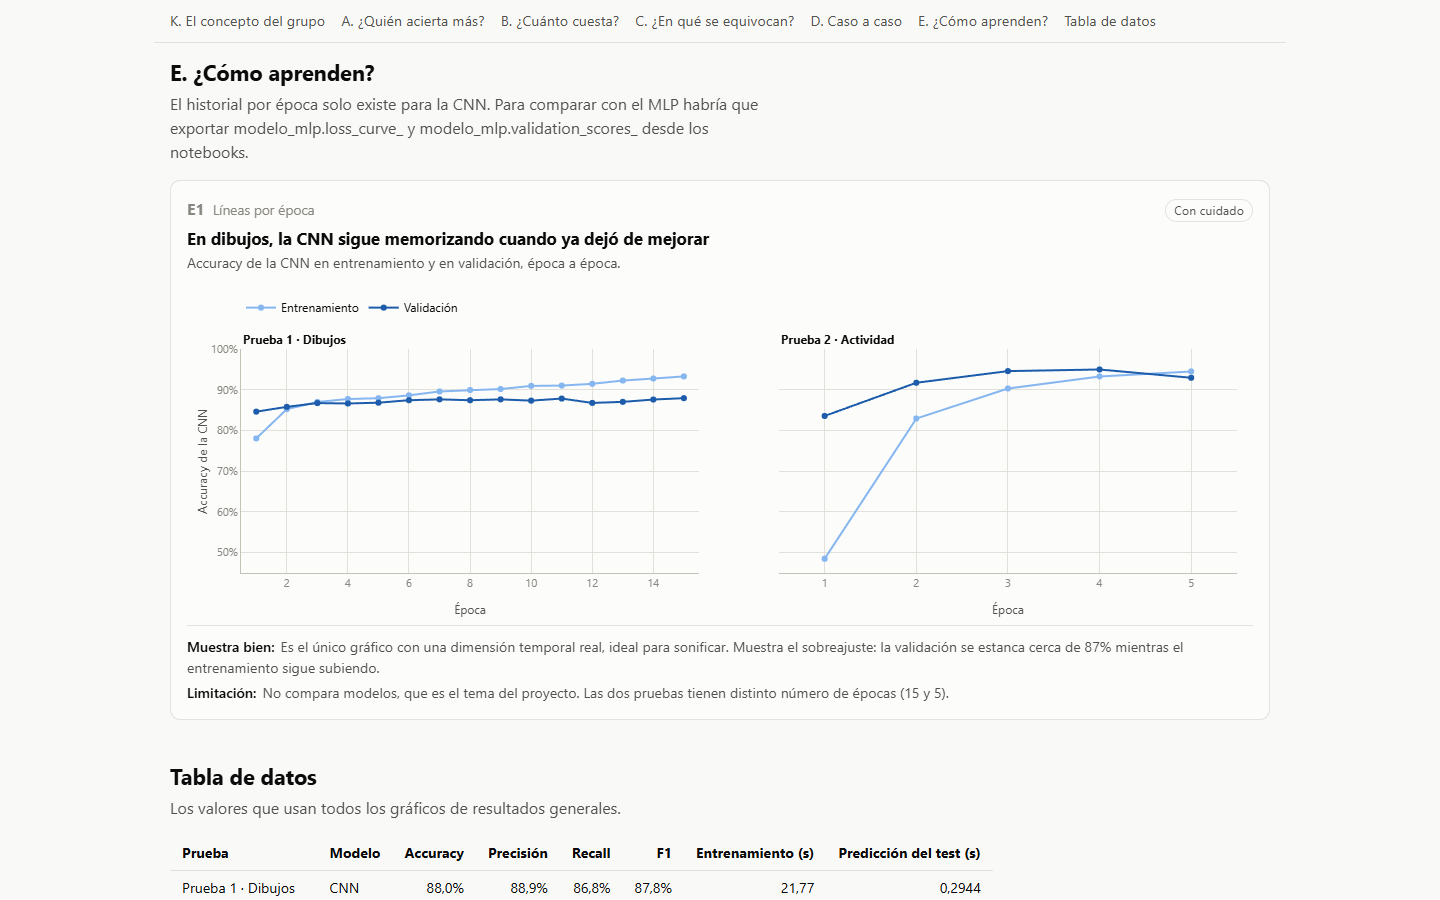
\includegraphics[width=\linewidth]{evidencia2/V2/v2_evolucion_entrenamiento.png}
\end{center}

{\centering
  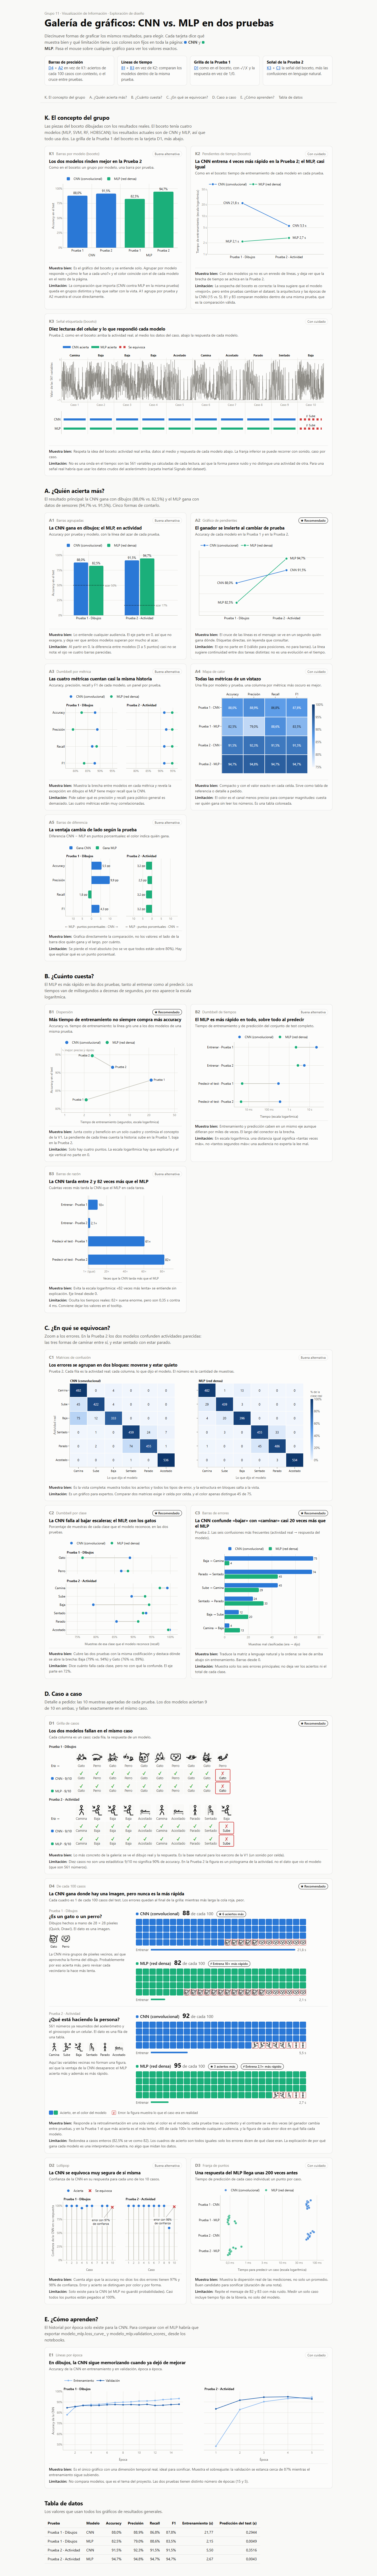
\includegraphics[width=0.95\linewidth,trim=0 7881 0 0,clip]{evidencia2/V2/v2_galeria_completa.png}\par
  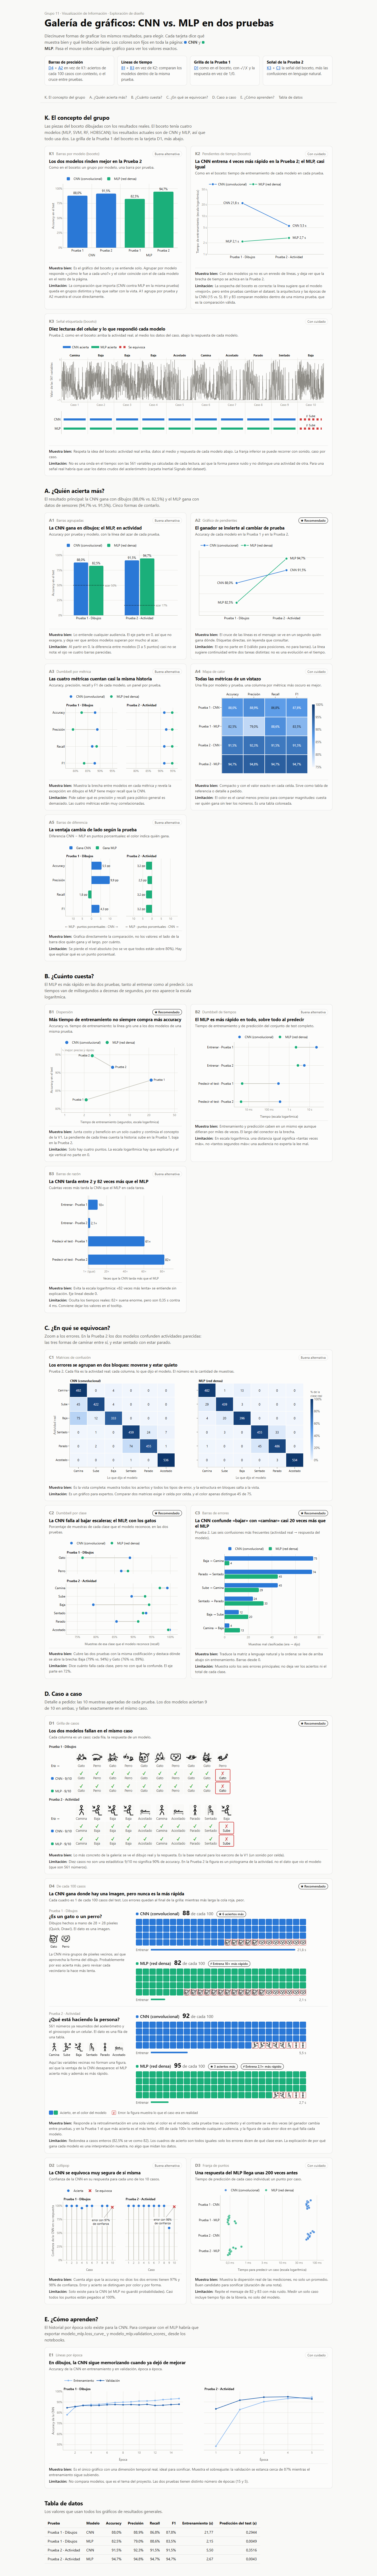
\includegraphics[width=0.95\linewidth,trim=0 5911 0 1970,clip]{evidencia2/V2/v2_galeria_completa.png}\par
  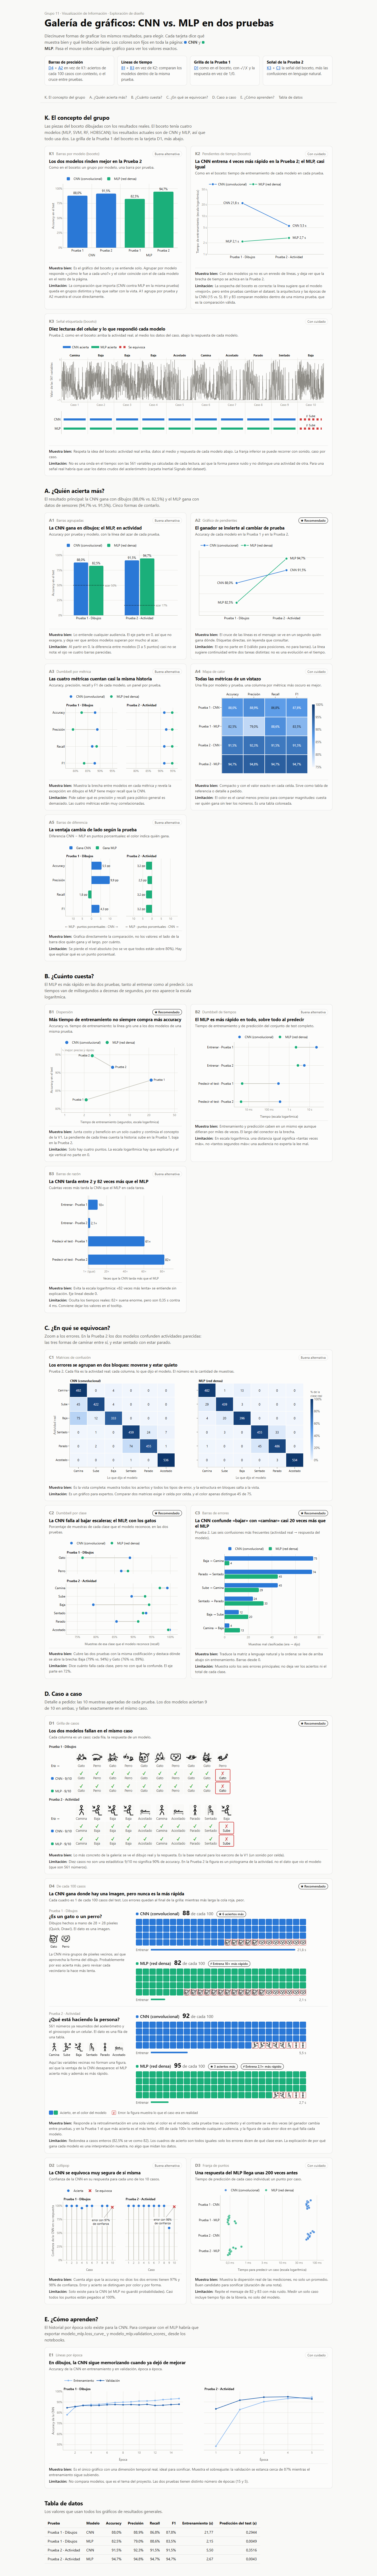
\includegraphics[width=0.95\linewidth,trim=0 3940 0 3940,clip]{evidencia2/V2/v2_galeria_completa.png}\par
  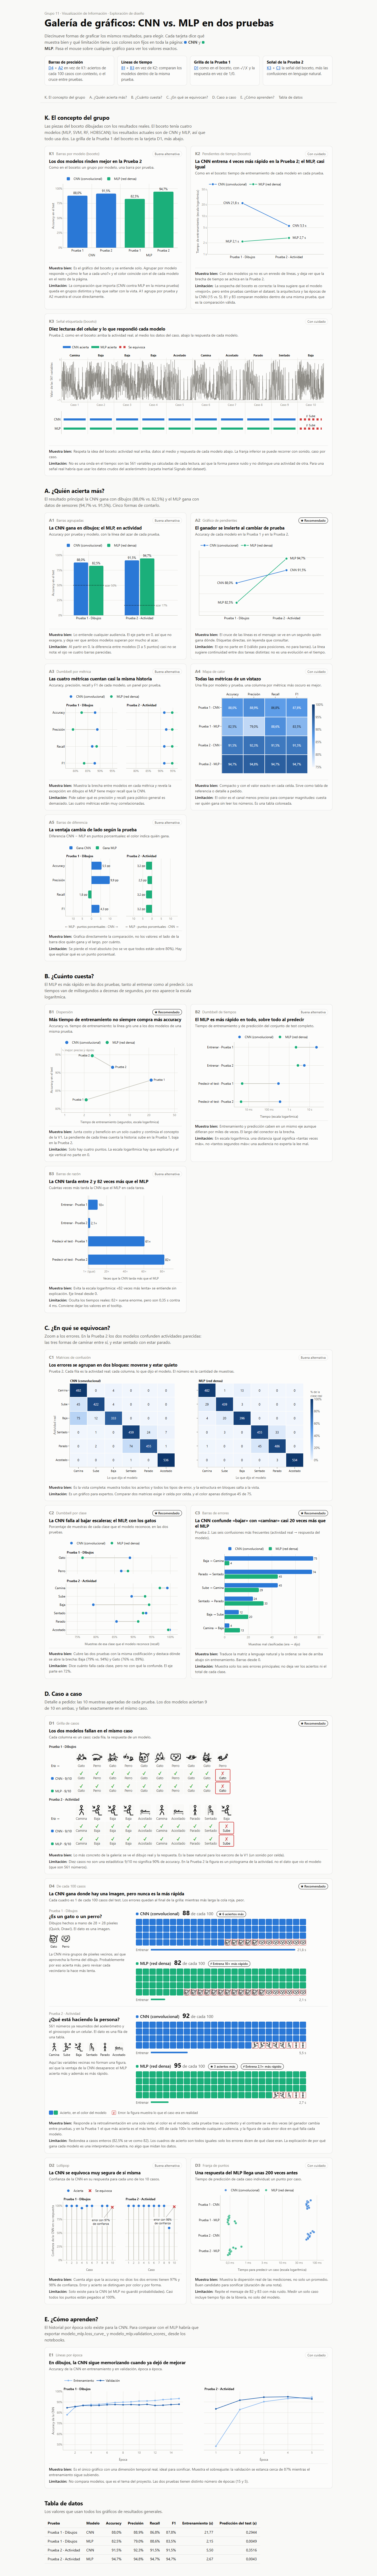
\includegraphics[width=0.95\linewidth,trim=0 1970 0 5911,clip]{evidencia2/V2/v2_galeria_completa.png}\par
  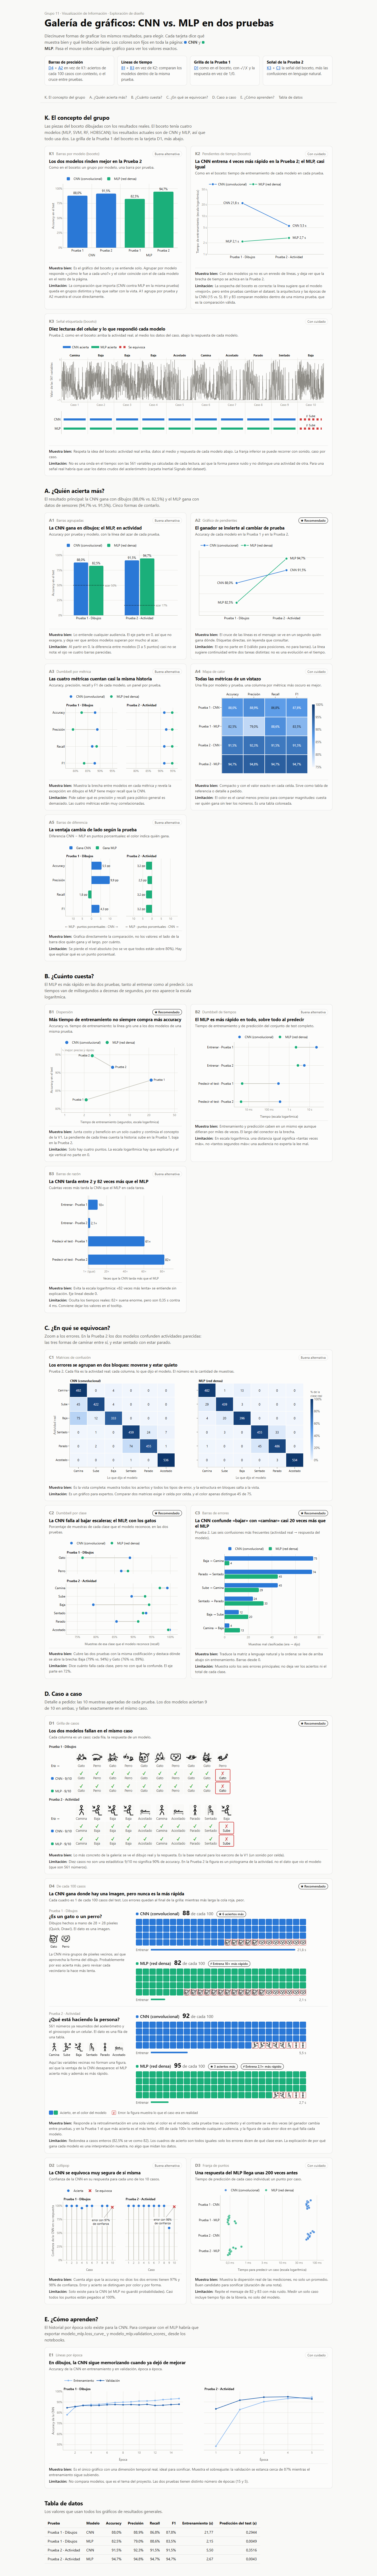
\includegraphics[width=0.95\linewidth,trim=0 0 0 7881,clip]{evidencia2/V2/v2_galeria_completa.png}\par
}

\noindent\textbf{Video} (click en la imagen para reproducirlo):
\begin{center}
  \href{https://josegdotcom.github.io/Proyecto-infovis/evidencia2/V2/grabacion_v2.mp4}{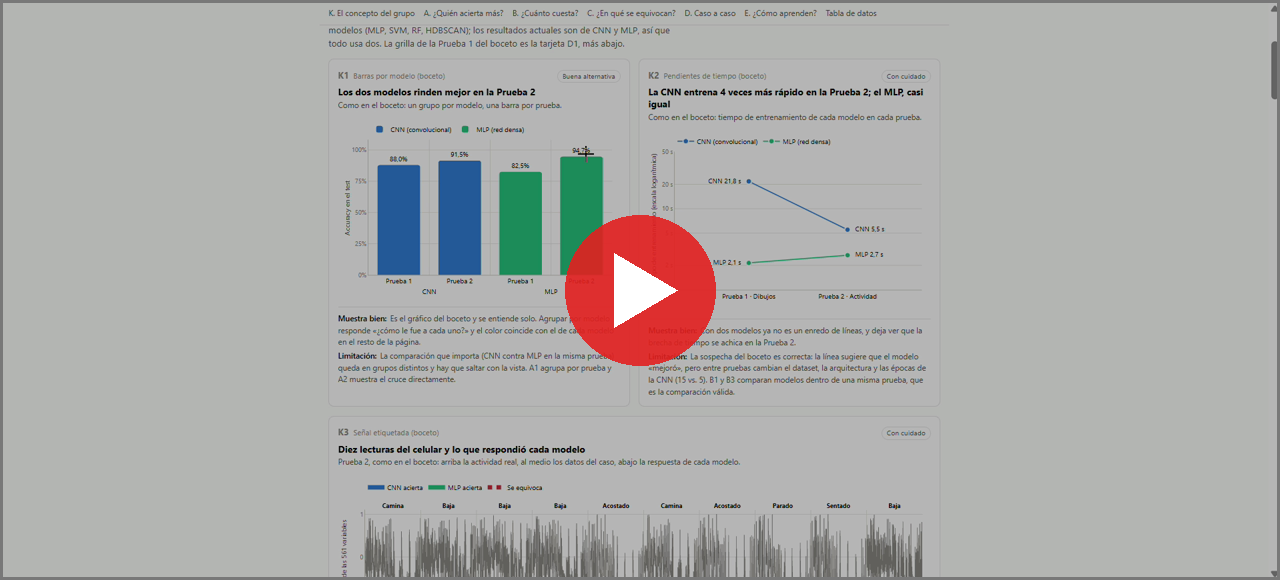
\includegraphics[width=0.85\linewidth]{evidencia2/V2/grabacion_v2_miniatura.png}}\\[0.3em]
  \small\url{https://josegdotcom.github.io/Proyecto-infovis/evidencia2/V2/grabacion_v2.mp4}
\end{center}

\subsection{Qu\'{e} cambi\'{o}}

Se incorpor\'{o} el segundo dataset (Human Activity Recognition) con sus notebooks de proceso
(\texttt{Proceso\_1.ipynb}, \texttt{Proceso\_2.ipynb}).
Se cre\'{o} la galer\'{i}a de exploraci\'{o}n (\texttt{exploracion/}) con 19 alternativas de
gr\'{a}ficos para ambas pruebas, generada con \texttt{data/exportar\_galeria.py}.
Tambi\'{e}n se a\~{n}adi\'{o} la visualizaci\'{o}n de evoluci\'{o}n del entrenamiento en el
tiempo.

\subsection{Por qu\'{e} cambi\'{o} (rationale)}

Con los resultados de la segunda prueba disponibles era necesario extender la visualizaci\'{o}n
para cubrir ambos experimentos de forma sim\'{e}trica.
La galer\'{i}a naci\'{o} como herramienta interna para elegir el tipo de gr\'{a}fico m\'{a}s
efectivo antes de comprometerse con un dise\~{n}o final.
La progresi\'{o}n temporal del entrenamiento agregaba una dimensi\'{o}n narrativa que
reforzaba el mensaje sobre las diferencias entre CNN y MLP.

\subsection{Qu\'{e} se descart\'{o}}

Se simplific\'{o} la estructura de archivos de resultados (NPZ individuales unificados).
El aplaus\'{o}metro de V1 qued\'{o} relegado frente al nuevo enfoque comparativo.

% =========================================================
\section{R2 --- revisi\'{o}n entre pares}
% =========================================================

\begin{tabular}{ll}
  \textbf{Fecha:} & {[SECCION PENDIENTE]} \\
\end{tabular}

\medskip
\noindent\textbf{S\'{i}ntesis de lo discutido:}

El otro grupo evalu\'{o} el proyecto de manera concreta y concisa.
Se se\~{n}al\'{o} que la idea central no se entend\'{i}a con facilidad a primera vista y que
se perd\'{i}a el eje del mensaje.
Tambi\'{e}n se observ\'{o} que los colores (azul y verde) no ten\'{i}an significado
sem\'{a}ntico m\'{a}s all\'{a} de diferenciar los modelos.
El sonido fue se\~{n}alado como decorativo en lugar de informativo.

\medskip
\noindent\textbf{Decisiones tomadas:}

\begin{itemize}
  \item \textbf{Adoptado:} Agregar un contexto r\'{a}pido en la p\'{a}gina que oriente al
        usuario antes de ver los gr\'{a}ficos.
  \item \textbf{Adoptado:} Redise\~{n}ar el sonido para que aporte informaci\'{o}n real
        (altura de nota = aciertos; duraci\'{o}n de pulsos = tiempo de entrenamiento;
        timbre y posici\'{o}n est\'{e}reo = modelo).
  \item \textbf{Descartado:} No se cambi\'{o} la paleta de colores (azul CNN / verde MLP),
        ya que la distinci\'{o}n por modelo se consider\'{o} suficiente.
\end{itemize}

% =========================================================
\section{V3 --- segunda iteraci\'{o}n de dise\~{n}o}
% =========================================================

\subsection{Identificaci\'{o}n}

\begin{tabular}{ll}
  \textbf{Fecha:}  & 7--8 de octubre de 2026 \\
  \textbf{Commit:} & \texttt{0fef4ab} --- cambio colores, tama\~{n}os de letra y contrastes \\
\end{tabular}

\subsection{Evidencia}

\begin{center}
  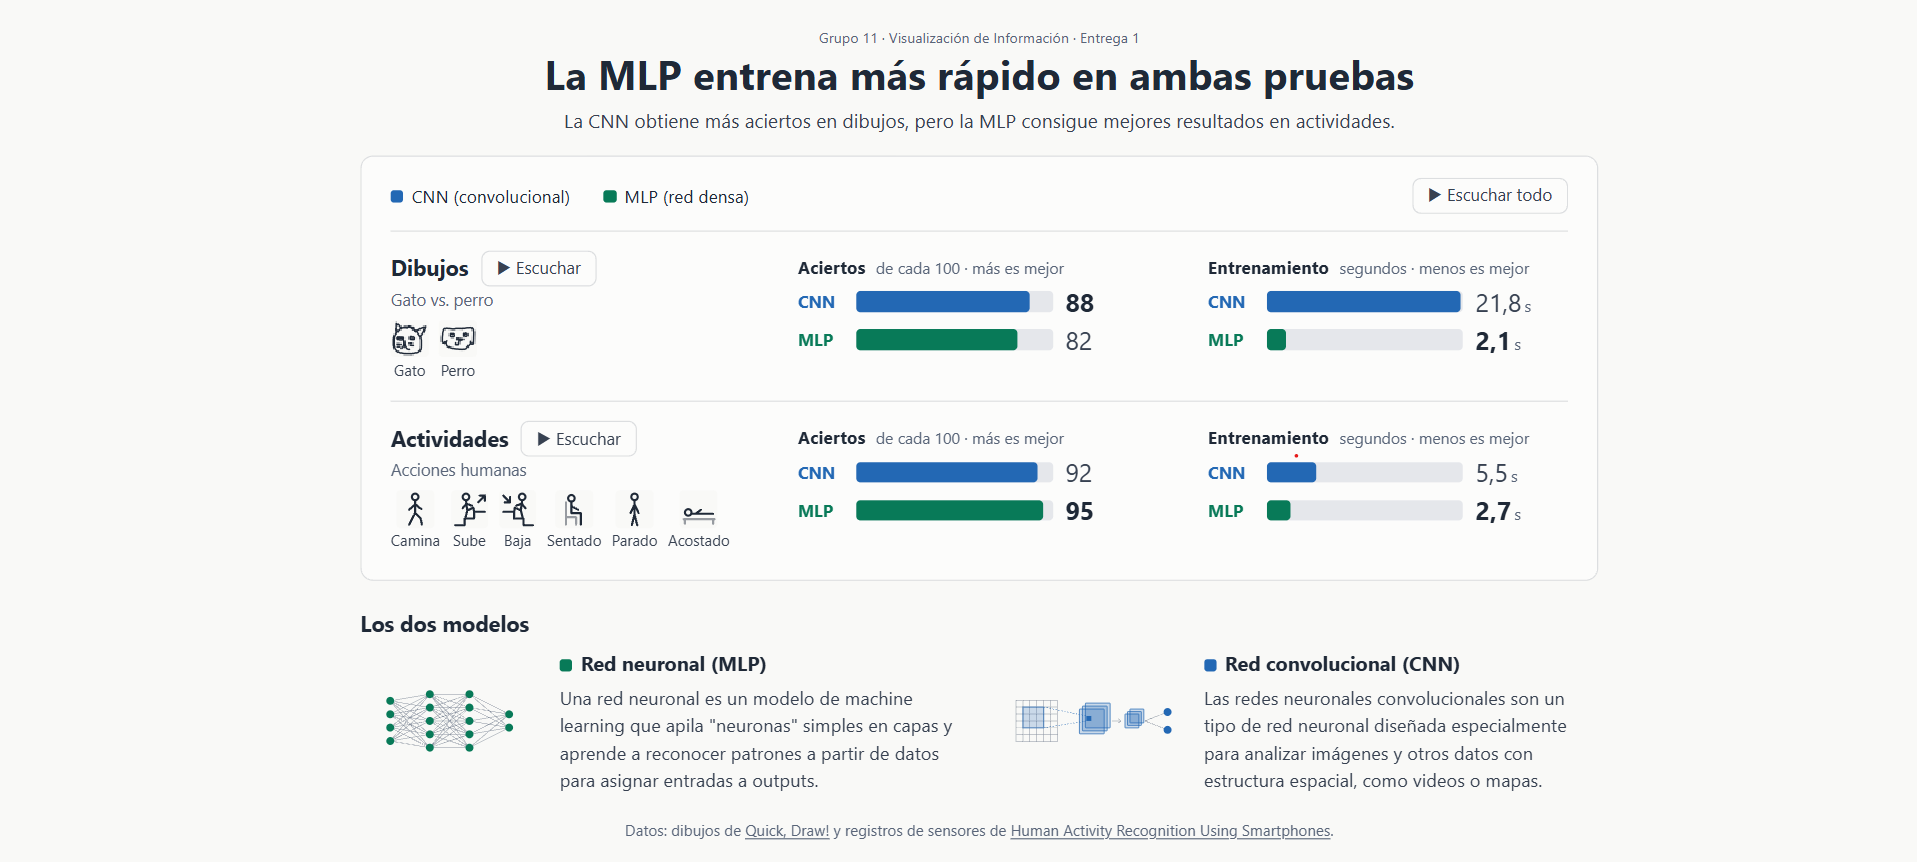
\includegraphics[width=\linewidth]{evidencia2/V3/imagen_v3.png}
\end{center}

\noindent\textbf{Video} (click en la imagen para reproducirlo):
\begin{center}
  \href{https://josegdotcom.github.io/Proyecto-infovis/evidencia2/V3/interaccion_v3.mp4}{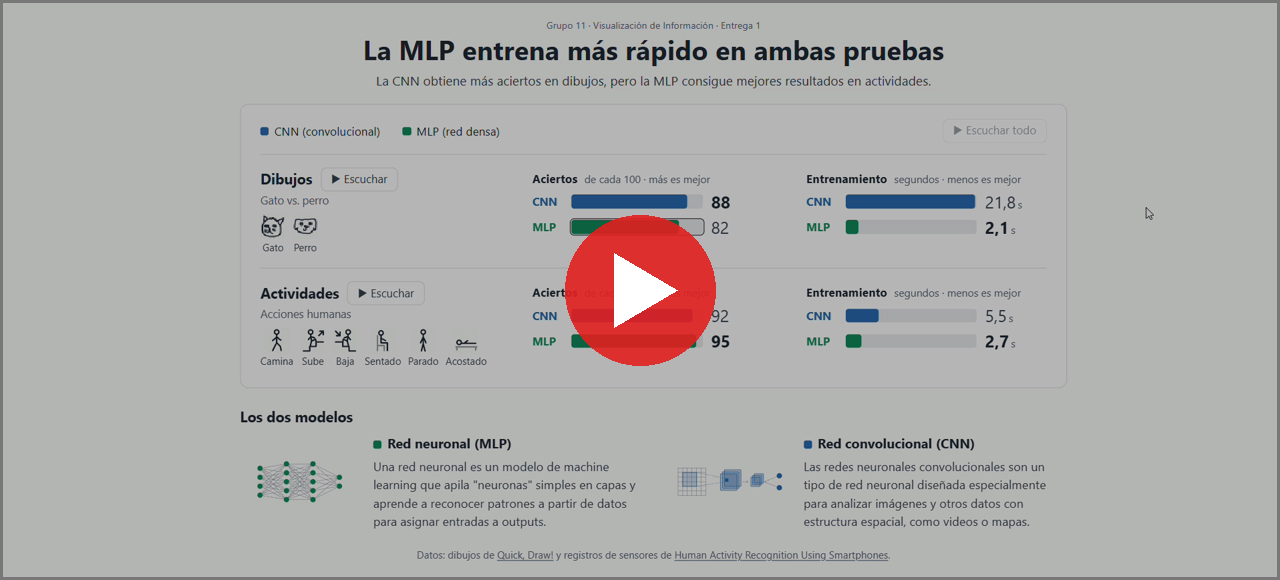
\includegraphics[width=0.85\linewidth]{evidencia2/V3/interaccion_v3_miniatura.png}}\\[0.3em]
  \small\url{https://josegdotcom.github.io/Proyecto-infovis/evidencia2/V3/interaccion_v3.mp4}
\end{center}

\subsection{Qu\'{e} cambi\'{o}}

Se construy\'{o} el gr\'{a}fico de barras comparativo definitivo
(\texttt{exploracion/comparacion.html} y \texttt{comparacion.js}) y se integr\'{o} la
sonificaci\'{o}n completa con Tone.js: altura de nota para aciertos, duraci\'{o}n de pulsos
para tiempo de entrenamiento, y timbre y posici\'{o}n est\'{e}reo para distinguir CNN
(izquierda) de MLP (derecha).
Se reorganiz\'{o} la l\'{o}gica de estilos en \texttt{css/comparacion.css} y se aplicaron
correcciones de contraste y tipograf\'{i}a.

\subsection{Por qu\'{e} cambi\'{o} (rationale)}

Tras la R2 qued\'{o} claro que el sonido deb\'{i}a ser informativo y no decorativo, lo que
motiv\'{o} el dise\~{n}o con Tone.js mapeando cada dimensi\'{o}n de datos a un par\'{a}metro
sonoro distinto.
El gr\'{a}fico de barras comparativo fue elegido de la galer\'{i}a exploratoria como el tipo
de visualizaci\'{o}n que comunicaba mejor la comparaci\'{o}n entre modelos y pruebas.
Las correcciones de contraste respondieron a est\'{a}ndares de accesibilidad.

\subsection{Qu\'{e} se descart\'{o}}

Se eliminaron los archivos de imagen temporales (\texttt{assets/icons/a1.png}, \texttt{a2.png})
usados en pruebas. Se descart\'{o} el aplaus\'{o}metro como forma de interacci\'{o}n principal.

% =========================================================
\section{R3 --- revisi\'{o}n con el equipo docente}
% =========================================================

\begin{tabular}{ll}
  \textbf{Fecha:} & {[SECCION PENDIENTE]} \\
\end{tabular}

\medskip
\noindent\textbf{S\'{i}ntesis de lo discutido:}

{[SECCION PENDIENTE]}

\medskip
\noindent\textbf{Decisiones tomadas:}

{[SECCION PENDIENTE]}

% =========================================================
\section{V4 --- la versi\'{o}n final}
% =========================================================

\subsection{Identificaci\'{o}n}

\begin{tabular}{ll}
  \textbf{Fecha:}  & 12 de octubre de 2026 \\
  \textbf{Commit:} & \texttt{56b63dd} --- Merge PR \#5 (codex/diseno-comparativa) \\
\end{tabular}

\subsection{Evidencia}

\begin{center}
  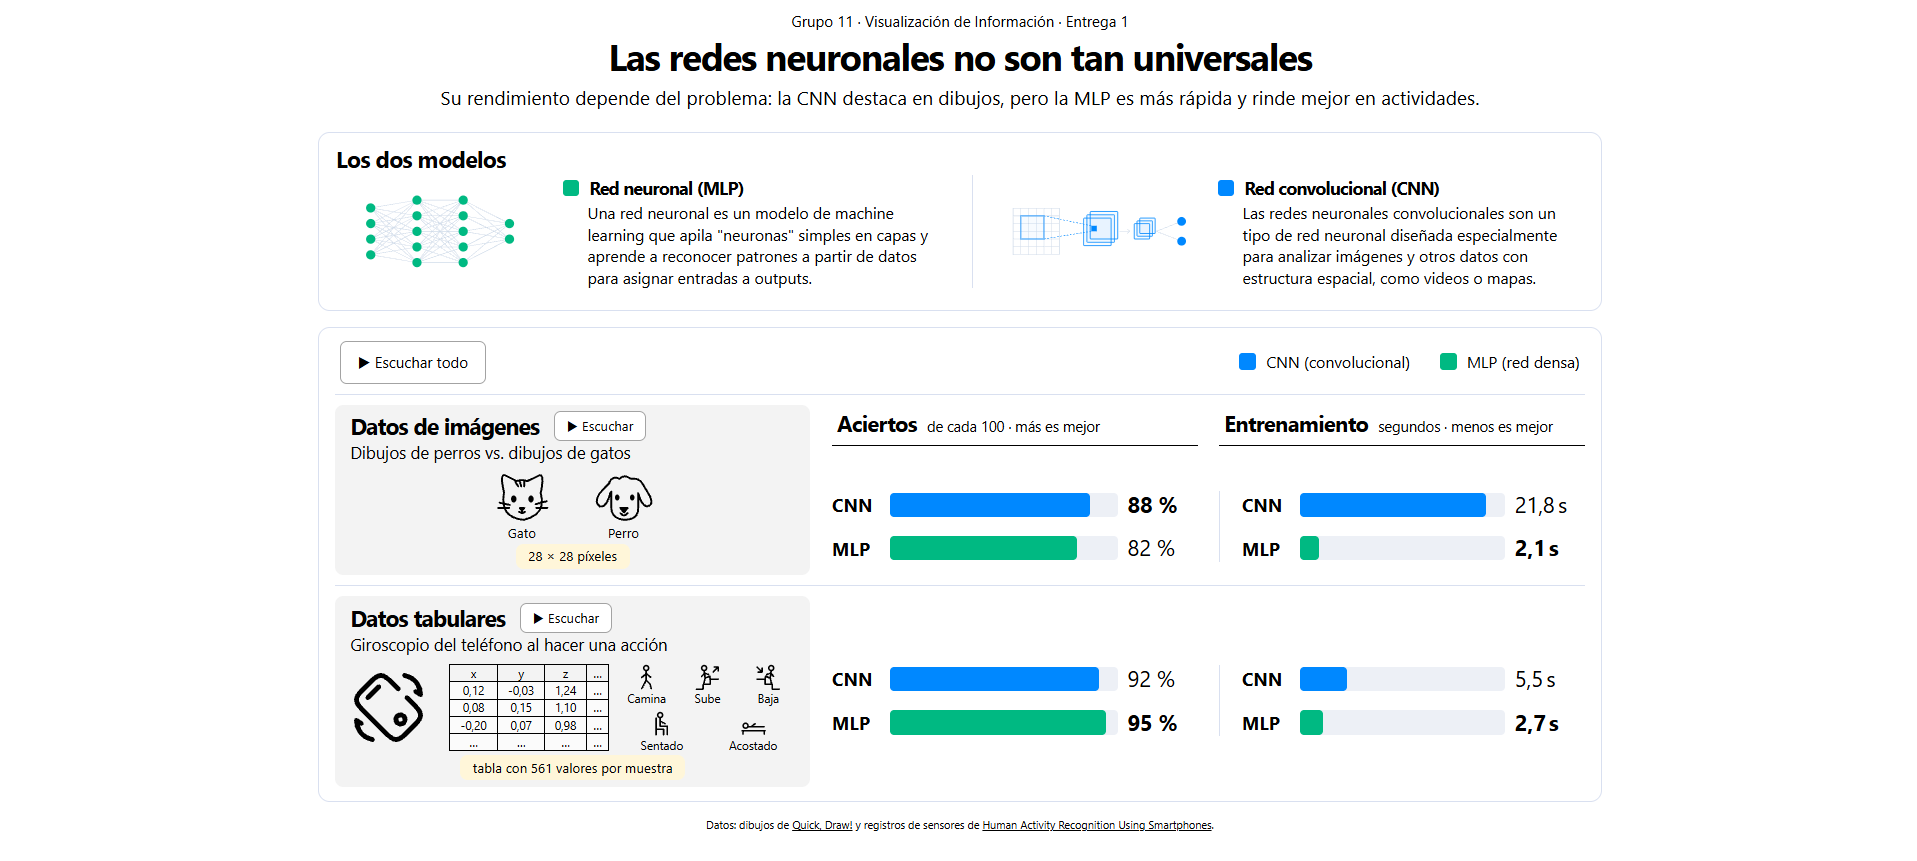
\includegraphics[width=\linewidth]{evidencia2/V4/imagen_v4.png}
\end{center}

\noindent\textbf{Video} (click en la imagen para reproducirlo):
\begin{center}
  \href{https://josegdotcom.github.io/Proyecto-infovis/evidencia2/V4/interaccion_v4.mp4}{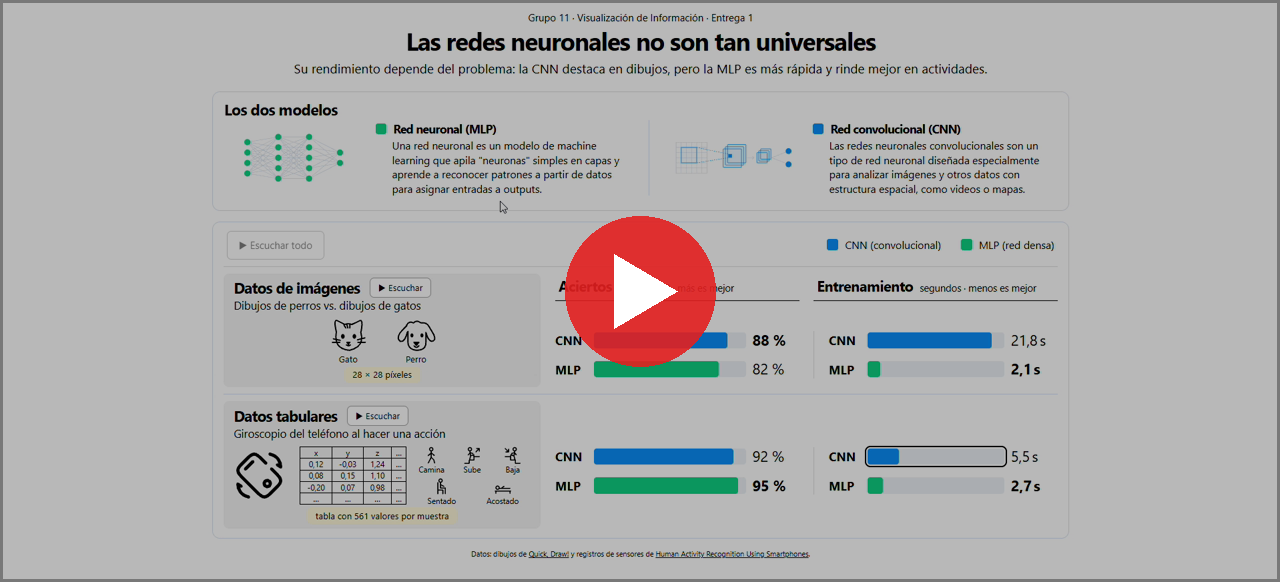
\includegraphics[width=0.85\linewidth]{evidencia2/V4/interaccion_v4_miniatura.png}}\\[0.3em]
  \small\url{https://josegdotcom.github.io/Proyecto-infovis/evidencia2/V4/interaccion_v4.mp4}
\end{center}

\subsection{Qu\'{e} cambi\'{o}}

Se ampli\'{o} la explicaci\'{o}n del experimento de actividades humanas y se agreg\'{o} el
\'{i}cono SVG \texttt{rotate\_phone.svg} para contextualizarlo.
Se aplic\'{o} un redise\~{n}o profundo del CSS: simplificaci\'{o}n de
\texttt{css/comparacion.css} y \texttt{css/style.css} (reducci\'{o}n de \texttildelow{}715
l\'{i}neas), eliminando estilos redundantes.
Se incorporaron los pictogramas SVG \texttt{gato.svg} y \texttt{perro.svg}, y se
actualizaron las fuentes bibliogr\'{a}ficas.

\subsection{Por qu\'{e} cambi\'{o} (rationale)}

La revisi\'{o}n interna (PR~\#4 y~\#5) identific\'{o} que la secci\'{o}n de actividades
humanas carec\'{i}a de contexto suficiente para el usuario no experto.
El redise\~{n}o del CSS respondi\'{o} a la necesidad de consolidar estilos dispersos en
m\'{u}ltiples archivos tras varias iteraciones r\'{a}pidas.
Los pictogramas SVG reemplazaron descripciones textuales para hacer la p\'{a}gina m\'{a}s
intuitiva y visual.

\subsection{Qu\'{e} se descart\'{o}}

Se eliminaron estilos duplicados y reglas CSS en desuso acumuladas durante las iteraciones
anteriores. La galer\'{i}a de exploraci\'{o}n qued\'{o} como secci\'{o}n secundaria.

% =========================================================
\section{El feedback al otro grupo (R2)}
% =========================================================

\subsection{El proyecto evaluado}

El \textbf{Grupo 20} desarroll\'{o} una visualizaci\'{o}n sobre la afluencia en el metro de
Santiago a las distintas horas del d\'{i}a.
Al momento de la evaluaci\'{o}n el proyecto mostraba un avance considerable para el tiempo que
llevaba de desarrollo: p\'{a}gina interactiva con sonidos y colores llamativos que comunicaban
la densidad de pasajeros de forma directa.

\subsection{El feedback que dimos}

Vimos una p\'{a}gina sobre la afluencia en el metro, bastante interactiva con sonidos
interesantes y colores muy visuales.
Los \'{u}nicos detalles que encontramos para se\~{n}alar fueron algunos \'{i}conos demasiado
peque\~{n}os que conten\'{i}an datos relevantes y que deber\'{i}an destacarse m\'{a}s
visualmente para no perderse en la interfaz.
En general el proyecto estaba bien encaminado y con una propuesta s\'{o}lida de sonificaci\'{o}n
e interacci\'{o}n.

\subsection{Lo que nos llevamos para nuestro proyecto}

Del proyecto del Grupo 20 nos llevamos aprendizajes sobre c\'{o}mo el color puede usarse de
forma sem\'{a}ntica junto con el sonido para reforzar el mensaje, y c\'{o}mo las interacciones
del usuario pueden gatillar respuestas audiovisuales que hagan la experiencia m\'{a}s inmersiva
e informativa.

% =========================================================
\section{Evaluaci\'{o}n con usuarios}
% =========================================================

{[SECCION PENDIENTE]}

\subsection{Ronda 1}

\subsubsection{Qui\'{e}n fue el pensador y cu\'{a}ndo}

{[SECCION PENDIENTE]}

\subsubsection{Bit\'{a}cora}

\begin{longtable}{p{2.5cm} p{5cm} p{5cm}}
  \toprule
  \textbf{Tiempo} & \textbf{Cita literal} & \textbf{Acci\'{o}n} \\
  \midrule
  \endhead
  {[T]} & {[SECCION PENDIENTE]} & {[SECCION PENDIENTE]} \\
  \bottomrule
\end{longtable}

\subsubsection{Qu\'{e} dijo del sonido}

{[SECCION PENDIENTE]}

\subsubsection{Heur\'{i}sticas que fallaron}

{[SECCION PENDIENTE]}

\subsubsection{Las tres respuestas de cierre}

\begin{itemize}
  \item \textbf{Atasco:} {[SECCION PENDIENTE]}
  \item \textbf{Hip\'{o}tesis equivocada:} {[SECCION PENDIENTE]}
  \item \textbf{Cambio concreto:} {[SECCION PENDIENTE]}
\end{itemize}

\subsubsection{Efecto en el proceso}

{[SECCION PENDIENTE]}

\end{document}
